\paragraph{Sơ đồ tuần tự Luồng nhắn tin văn bản qua SSE}

Luồng nghiệp vụ này mô tả vòng đời của một yêu cầu chat văn bản từ Web Frontend tới Conversation Service, qua Chatbot Service bằng gRPC streaming và trả kết quả về client bằng Server-Sent Events (SSE). Luồng bao gồm kiểm tra quyền VIP khi bật reasoning, kiểm tra phiên chat active, truyền token qua gRPC metadata, stream các gói \texttt{status}, \texttt{content}, \texttt{metadata}, đồng thời lưu lịch sử chat ở Chatbot Service.

\begin{figure}[H]
\centering
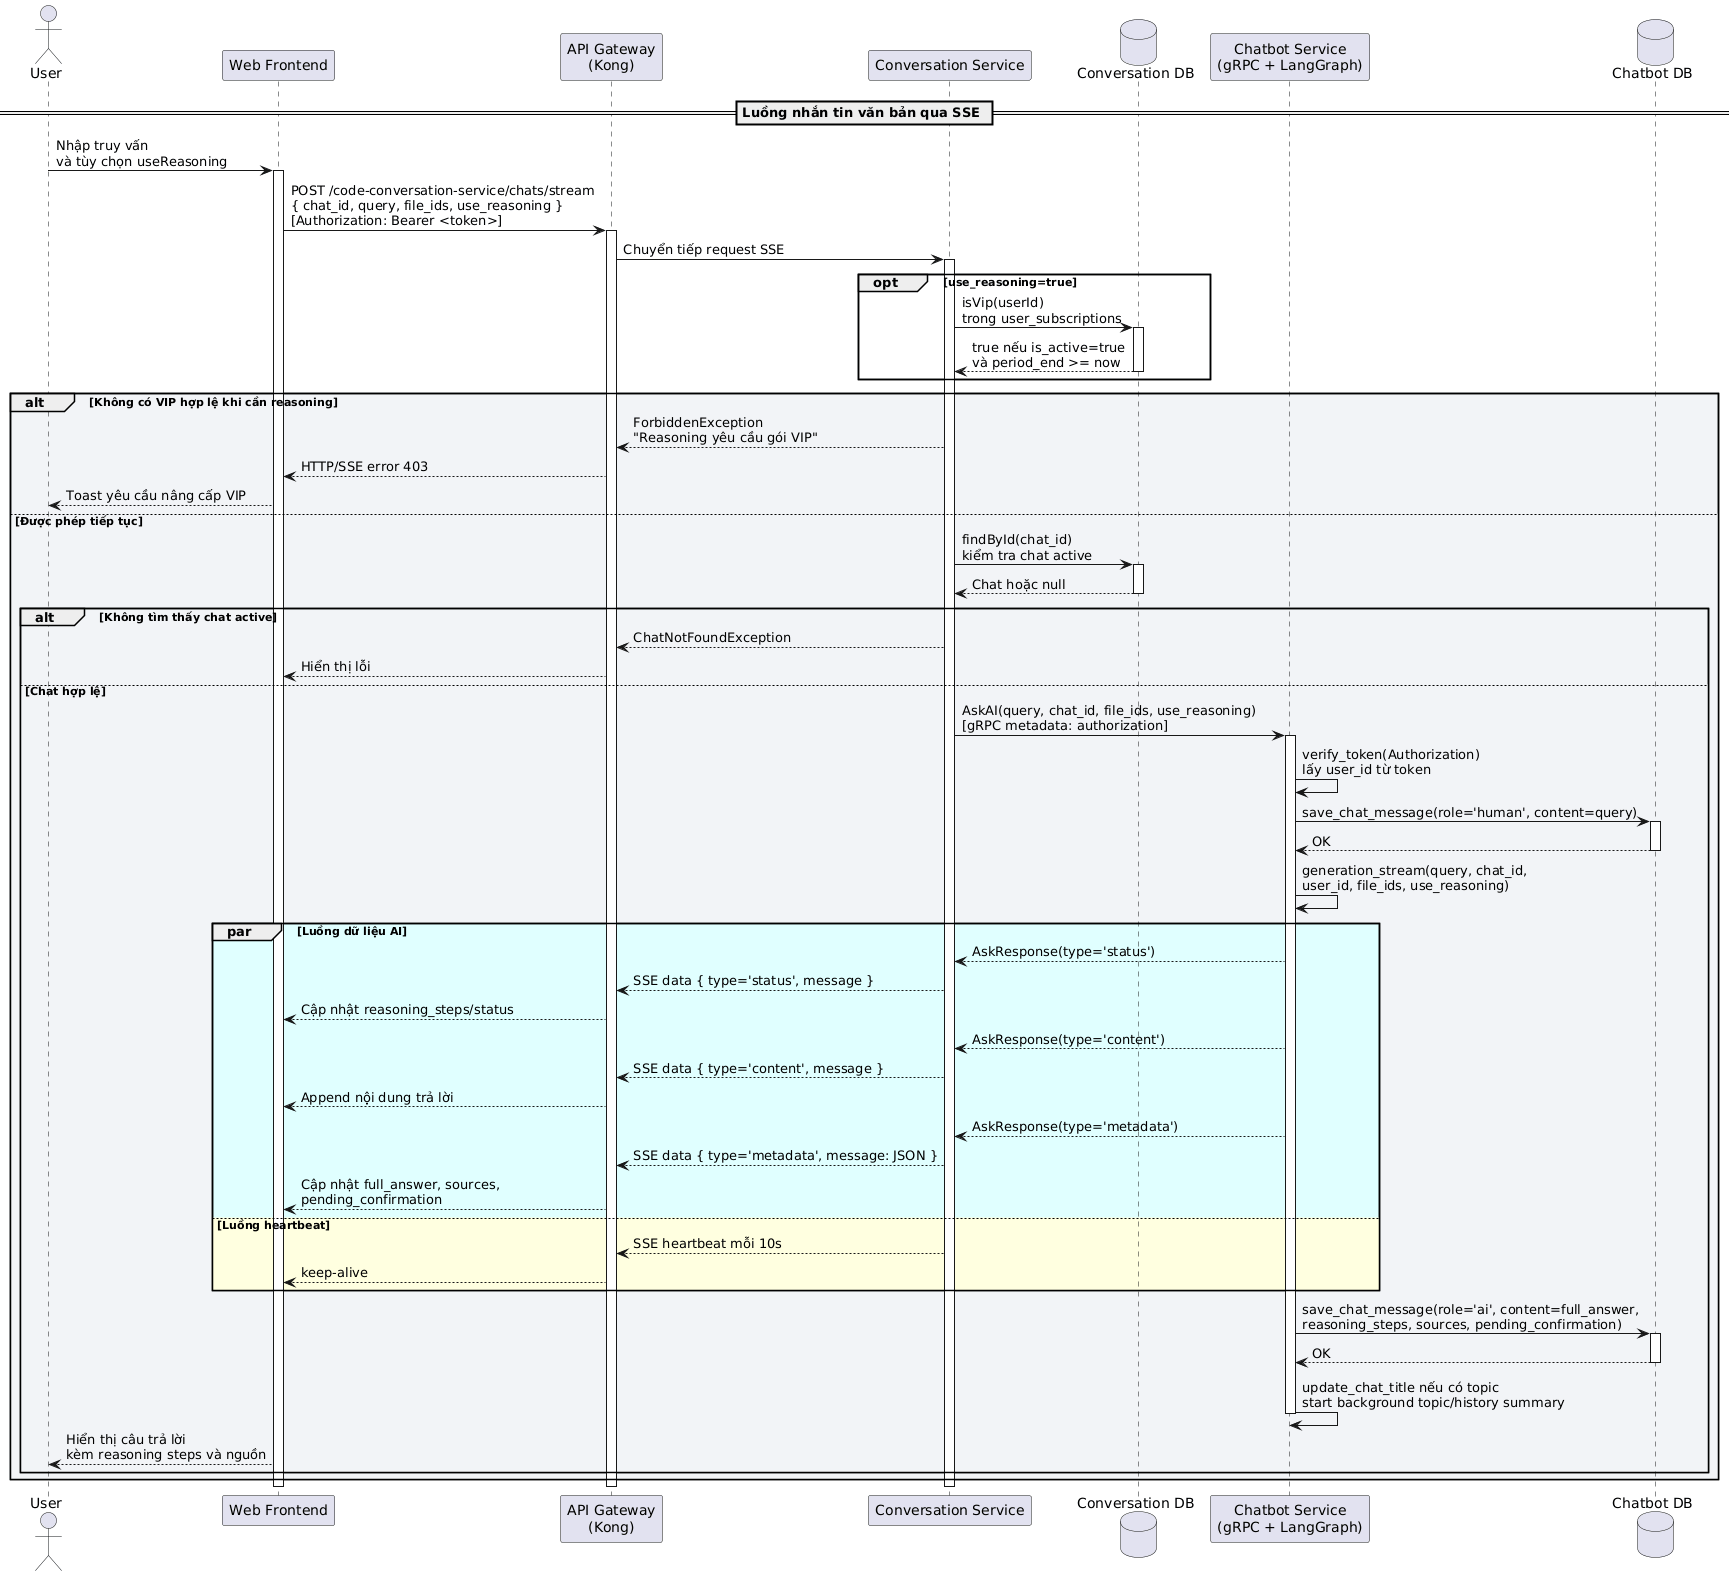
\includegraphics[scale = 0.18]{contents/Sequence/UML-Sequence-UserTextChatSse.png}
\caption{Sơ đồ tuần tự Luồng nhắn tin văn bản qua SSE}
\end{figure}

\subparagraph{Các thành phần tham gia}

\begin{table}[H]
\centering
\renewcommand{\arraystretch}{1.3}
\begin{tabular}{|l|l|p{5cm}|}
\hline
\textbf{Thành phần} & \textbf{Phân loại} & \textbf{Vai trò trong hệ thống} \\ \hline
User & Actor & Người dùng nhập truy vấn, chọn tài liệu đính kèm và tùy chọn bật reasoning. \\ \hline
Web Frontend & Component & Giao diện web Next.js. \\ \hline %%%% Component & Gọi \texttt{conversationService.streamChat}, xử lý SSE và hiển thị status, nội dung, reasoning steps, sources. \\ \hline
API Gateway (Kong) & Component & Cổng API chuyển tiếp các yêu cầu API. \\ \hline %%%% Component & Định tuyến request stream có Bearer Token tới Conversation Service. \\ \hline
Conversation Service & Microservice & Kiểm tra quyền VIP khi cần, kiểm tra chat active, mở SSE stream và gọi Chatbot Service qua gRPC. \\ \hline
Conversation DB & Database & Lưu chat session và bảng \texttt{user\_subscriptions} dùng để kiểm tra VIP. \\ \hline
Chatbot Service (gRPC + LangGraph) & Microservice & Verify token từ gRPC metadata, xử lý RAG/reasoning, stream kết quả và lưu lịch sử chat. \\ \hline
Chatbot DB & Database & Lưu human message, AI message, reasoning steps, sources và trạng thái xác nhận. \\ \hline
\end{tabular}
\caption{Các thành phần tham gia luồng nhắn tin văn bản qua SSE}
\end{table}

\subparagraph{Mô tả tổng quan}
\begin{itemize}
\item \textbf{Gửi yêu cầu stream:} Frontend gọi \texttt{POST /code-conversation-service/chats/stream} với \texttt{chat\_id}, \texttt{query}, \texttt{file\_ids}, \texttt{use\_reasoning} và Bearer Token.
\item \textbf{Kiểm tra VIP:} Khi \texttt{use\_reasoning=true} và môi trường không phải \texttt{development}, Conversation Service gọi \texttt{isVip(userId)} trên bảng \texttt{user\_subscriptions}. Subscription hợp lệ khi \texttt{is\_active=true} và \texttt{period\_end >= now}; nếu không hợp lệ, service trả \texttt{ForbiddenException}.
\item \textbf{Kiểm tra chat:} Conversation Service kiểm tra \texttt{findById(chat\_id)} để đảm bảo phiên chat còn active; nếu không có thì trả \texttt{ChatNotFoundException}.
\item \textbf{Gọi Chatbot Service:} Conversation Service gọi gRPC \texttt{AskAI(query, chat\_id, file\_ids, use\_reasoning)} và truyền token qua metadata \texttt{authorization}.
\item \textbf{Streaming kết quả:} Chatbot Service verify token, lưu human message, gọi \texttt{generation\_stream}, rồi stream các gói \texttt{status}, \texttt{content} và \texttt{metadata}. Controller chuyển chúng thành SSE; Frontend cập nhật reasoning steps, nội dung, \texttt{full\_answer}, sources và \texttt{pending\_confirmation}.
\item \textbf{Lưu lịch sử:} Khi có câu trả lời cuối, Chatbot Service lưu AI message kèm \texttt{reasoning\_steps}, sources và \texttt{pending\_confirmation}, sau đó cập nhật topic hoặc chạy background task tóm tắt lịch sử nếu cần.
\end{itemize}
